% \subsection{Numeric results and timings}\label{sec:truncation_effect}


% \graphicspath{{chapters/03_queueing_model/img/numeric_results_and_timings/}}

% \subsubsection{Markov chain waiting time approaches comparison}
% \label{sec:waiting_time_approach_comparison}

% In Section \ref{sec:waiting_time} three different approaches for calculating
% the waiting time using the Markov chain model have been introduces.
% The three approaches are the recursive approach, the direct approach and
% the closed form approach.
% In this section the three approaches are compared in terms of accuracy and
% computation time.

% In terms of accuracy the three approaches get close to identical results.
% Figures~\ref{fig:waiting_time_accuracy_over_N} and
% \ref{fig:waiting_time_accuracy_over_M} show the differences of the three
% approaches for different values of \(N\) and \(M\).


% \begin{figure}[H]
%     \includegraphics[width=12cm]{waiting_time_formulas_comparison/waiting_time_over_N.png}
%     \caption{Waiting times of the three waiting time approaches for different
%     values of \(N\).}
%     \label{fig:waiting_time_accuracy_over_N}
% \end{figure}
    
% \begin{figure}[H]
%     \includegraphics[width=12cm]{waiting_time_formulas_comparison/waiting_time_over_M.png}
%     \caption{Waiting times of the three waiting time approaches for different
%     values of \(M\).}
%     \label{fig:waiting_time_accuracy_over_M}
% \end{figure}


% Since the results of the three approaches are almost identical, the computation
% time of the three approaches is the main factor that determines which
% approach will be used.
% Figures~\ref{fig:waiting_time_algorithm_duration_over_N}, 
% \ref{fig:waiting_time_algorithm_duration_over_M} and 
% \ref{fig:waiting_time_algorithm_duration_over_N_and_M} show the computation
% time needed to calculate the waiting time for different values of \(N\) and
% \(M\).

% \begin{figure}[H]
%     \includegraphics[width=12cm]{waiting_time_formulas_comparison/algorithm_duration_over_N.png}
%     \caption{Duration of the three waiting time approaches for different values
%     of \(N\).}
%     \label{fig:waiting_time_algorithm_duration_over_N}
% \end{figure}

% \begin{figure}[H]
%     \includegraphics[width=12cm]{waiting_time_formulas_comparison/algorithm_duration_over_M.png}
%     \caption{Duration of the three waiting time approaches for different values
%     of \(M\).}
%     \label{fig:waiting_time_algorithm_duration_over_M}
% \end{figure}


% \begin{figure}[H]
%     \includegraphics[width=12cm]{waiting_time_formulas_comparison/algorithm_duration_over_N_and_M.png}
%     \caption{Duration of the three waiting time approaches for different values
%     of \(N\) and \(M\).}
%     \label{fig:waiting_time_algorithm_duration_over_N_and_M}
% \end{figure}

% The direct approach is the slowest approach, which makes sense since it requires
% solving a system of linear equations.
% The recursive approach and the closed form approach give similar durations,
% although the recursive approach seems to be more linear in nature than the
% closed form method. 


% \subsubsection{Markov chain - Simulation comparison of steady state probabilities}

% Another comparison that can be made is the comparison between the steady state
% probabilities calculated using the Markov chain and the simulation.
% The steady state probabilities, defined in
% Section~\ref{sec:steady_state_probabilities}, are an essential measure since
% they are necessary in the calculation of all performance measures using the
% Markov chain model.
% Although, there is no need to calculate the steady state probabilities for the
% simulation, it is interesting to see how the two approaches compare.
% Figures~\ref{fig:comparison_steady_state_probabilities_1}
% to~\ref{fig:comparison_steady_state_probabilities_5} show a comparison between
% the steady state probabilities between the Markov chain and the simulation
% for different values of \(\mu\).
% The value of \(\mu\) gradually increases from \(\mu = 0.03\) to \(\mu = 0.27\)
% and for each one three plots are generated; the steady state probabilities
% generated by the Markov chain, the steady state probabilities generated by the
% simulation and the difference between the two.
% The rest of the parameters have the following values:

% \begin{multicols}{2}
%     \begin{itemize}
%         \item \(\lambda_1\) = 0.3
%         \item \(\lambda_2\) = 0.3
%         \item \(C\) = 5
%         \item \(T\) = 5
%         \item \(N\) = 20
%         \item \(M\) = 20
%     \end{itemize}    
% \end{multicols}


% \begin{figure}[H]
%     \includegraphics[width=\textwidth, trim=200 60 170 60, clip]{steady_state_probabilities/main_1.png}
%     \caption{\(\mu = 0.03\)}
%     \label{fig:comparison_steady_state_probabilities_1}
% \end{figure}

% \begin{figure}[H]
%     \includegraphics[width=\textwidth, trim=200 60 170 60, clip]{steady_state_probabilities/main_3.png}
%     \caption{\(\mu = 0.09\)}
%     \label{fig:comparison_steady_state_probabilities_2}
% \end{figure}

% \begin{figure}[H]
%     \includegraphics[width=\textwidth, trim=200 60 170 60, clip]{steady_state_probabilities/main_5.png}
%     \caption{\(\mu = 0.15\)}
%     \label{fig:comparison_steady_state_probabilities_3}
% \end{figure}

% \begin{figure}[H]
%     \includegraphics[width=\textwidth, trim=200 60 170 60, clip]{steady_state_probabilities/main_7.png}
%     \caption{\(\mu = 0.21\)}
%     \label{fig:comparison_steady_state_probabilities_4}
% \end{figure}

% \begin{figure}[H]
%     \includegraphics[width=\textwidth, trim=200 60 170 60, clip]{steady_state_probabilities/main_9.png}
%     \caption{\(\mu = 0.27\)}
%     \label{fig:comparison_steady_state_probabilities_5}
% \end{figure}

% Figure~\ref{fig:comparison_steady_state_probabilities_1} has the smallest
% value of \(\mu = 0.03\).
% It can be seen that for both the Markov chain and the simulation the steady
% state probabilities are close to zero for most states apart from the
% states close to when the system is full.
% That is because the arrival rate of individuals is much lower than the service
% rate of individuals even with 5 servers.
% Note here that because the model is immediately flooded from the beginning, the
% simulation has no time to explore the state space, so the heatmap looks like
% it is missing some of its pieces.
% Additionally, it is interesting to note that as we increase the value of \(\mu\)
% in Figures~\ref{fig:comparison_steady_state_probabilities_2} -
% \ref{fig:comparison_steady_state_probabilities_5} smaller states in the model
% have a higher value since individuals now exit the system faster.
% Also, note that for all values of \(\mu\) the difference between the Markov
% chain approach and the simulation is small.


% \subsubsection{Simulation VS Markov chain durations}

% The choice of the artificial parameters \(N\) and \(M\) is an important 
% decision of the model.
% In the untruncated simulation these values can be omitted by setting them to
% infinity.
% This is not possible when obtaining the steady state probabilities of the
% finite state Markov chain.
% The value of \(N\) and \(M\) can be chosen arbitrarily large, but the
% computation time increases as the size of the state space increases.
% Table \ref{tab:truncation_effect_timings_old} shows the relative timings of the
% different approaches used to get the performance measures for different values
% of \(N\) and \(M\).
% Note that \(N\) and \(M\) have the same value throughout the table.
% Simulation is ran for a runtime of \(10^4\) time units and the displayed
% durations are for a single run of the simulation and similarly for 100 runs of
% the simulation.
% For getting the performance measures using the finite state Markov chain each
% timing recorded is for the computation of the steady state probabilities and
% then the corresponding performance measure.

% \tiny
% \begin{table}[H]
%     \centering
%     \begin{tabular}{c|cc|ccc}
%         & \multicolumn{2}{c}{\textbf{Simulation}} & 
%         \multicolumn{3}{c}{\textbf{Markov chain}} \\
%         \textbf{Value of} & \textbf{Single} & \textbf{100} & 
%         \textbf{Waiting} & \textbf{Blocking} & 
%         \textbf{Proportion} \\
%         \textbf{\textit{N} and \textit{M}} & \textbf{trial} & \textbf{trials} & 
%         \textbf{formula} & \textbf{formula} & \textbf{formula} \\
%         \hline
%         \(10\) & 1 & 144.3 & 0.015  & 0.014  & 0.014 \\
%         \hline
%         \(30\) & 1 & 143.4 & 3.73   & 3.83   & 3.65 \\
%         \hline
%         \(50\) & 1 & 139.8 & 31.57  & 38.39  & 31.98 \\
%         \hline
%         \(\infty\) & 1 & 142.1 & N/A & N/A & N/A \\
%     \end{tabular}
%     \caption{Relative timings of the simulation and Markov chain model}
%     \label{tab:truncation_effect_timings_old}
% \end{table}
% \normalsize

% After some investigation it was found that a huge proportion of the duration of
% time needed to get the performance measures using the Markov chain approach is
% due to the creation of the generator matrix defined in
% equation~(\ref{eq:markov_transition_rate}).
% For example, for \(N = M = 50\) the state space of the Markov chain consists
% of approximately \(2500\) states (depending on the value of \(T\)).
% Thus, the generator matrix, that consists of the rates from each state to every
% other state, has approximately \(2500^2 = 6250000\) entries.
% For larger values of \(N\) and \(M\), the creation of this matrix is the most
% time consuming part of the Markov chain approach, even though most entries in
% the matrix are zero.
% By using equation~(\ref{eq:state_map_to_destination_states}), the set of states
% with a non-zero rate can be used to fill out the generator matrix.
% Thus, instead of iterating over the set states twice, the generator matrix can
% be filled out by iterating over the states only once and using
% \(\mathcal{M}(u,v)\) defined in
% equation~(\ref{eq:state_map_to_destination_states}).
% Table~\ref{tab:truncation_effect_timings_new} shows how the relative timings
% of the different approaches change when using this smarter approach.


% \tiny
% \begin{table}[H]
%     \centering
%     \begin{tabular}{c|cc|ccc}
%         & \multicolumn{2}{c}{\textbf{Simulation}} & 
%         \multicolumn{3}{c}{\textbf{Markov chain}} \\
%         \textbf{Value of} & \textbf{Single} & \textbf{100} & 
%         \textbf{Waiting} & \textbf{Blocking} & 
%         \textbf{Proportion} \\
%         \textbf{\textit{N} and \textit{M}} & \textbf{trial} & \textbf{trials} & 
%         \textbf{formula} & \textbf{formula} & \textbf{formula} \\
%         \hline
%         \(10\) & 1 & 119.2 & 0.000415 & 0.000146 & 0.000274 \\
%         \hline
%         \(30\) & 1 & 108.2 & 0.008040 & 0.035941 & 0.013451 \\
%         \hline
%         \(50\) & 1 & 109.3 & 0.147455 & 1.229303 & 0.179336 \\
%         \hline
%         \(\infty\) & 1 & 127.4 & N/A & N/A & N/A \\
%     \end{tabular}
%     \caption{Relative timings of the simulation and Markov chain model using
%     the smarter approach}
%     \label{tab:truncation_effect_timings_new}
% \end{table}
% \normalsize

% Overall, it can be seen that using the Markov chain approach is much faster than
% simulating the system.
% Although, by choosing a larger value of \(N\) and \(M\) the computation time of
% the Markov chain model increases while the simulation time stays relatively 
% similar.

% \subsubsection{Truncation effect on performance measures}

% This section is used to demonstrate the accuracy of the performance measure
% formulas of the constructed Markov model compared to the simulation as well as
% the effect of truncating the model.
% The simulation was run 100 times and the recorded mean waiting time at each
% iteration is used to populate the violin plots that are shown in
% Figures~\ref{fig:markov_vs_des_waiting_time_comparison_overall},
% \ref{fig:markov_vs_des_blocking_time_comparison_overall} and
% \ref{fig:markov_vs_des_proportion_within_time_comparison_overall}.

% Figure \ref{fig:markov_vs_des_waiting_time_comparison_overall} shows a 
% comparison between the calculated mean waiting time using Markov chains and the
% simulated waiting time using discrete event simulation over a range of values of 
% \(\lambda_2\) (details of the discrete event simulation model can be found in 
% Section~\ref{sec:discrete_event_simulation}).

% \begin{figure}[H]
%     \includegraphics[width=\textwidth]{truncation_effect/waiting/demo.pdf}
%     \caption{
%         Comparison of mean waiting time between values obtained from the Markov 
%         chain formula, values obtained from the truncated simulation and values
%         obtained from the untruncated simulation.
%     }
%     \label{fig:markov_vs_des_waiting_time_comparison_overall}
% \end{figure}

% In detail, Figure~\ref{fig:markov_vs_des_waiting_time_comparison_overall} shows
% the calculated mean waiting time using the Markov chain, using a truncated 
% simulation and using a simulation with infinite capacity (without the artificial
% parameters \(N\) and \(M\)).
% Each plot corresponds to different values of \(N\) and \(M\) and is run over 
% different values of \(\lambda_2\).
% The untruncated simulation values are the same at all three graphs since
% the effect of truncation does not apply to it.
% The waiting times generated by the truncated simulation match the ones generated 
% by the Markov chains model.
% Note that this comparison includes both type 1 and type 2 individuals.
% % TODO: Include type 1 and type 2 plot?


% Similarly Figure~\ref{fig:markov_vs_des_blocking_time_comparison_overall} shows
% the mean blocking time equivalent comparison between the three approaches used
% for the waiting time (Markov chain, truncated simulation and untruncated
% simulation).
% Similar to the waiting time, the blocking time among the different approaches
% begin to get closer together as the value of \(N\) and \(M\) increases.
% Note that the blocking time can only be calculated for type 2 individuals.

% \begin{figure}[H]
%     \includegraphics[width=\textwidth]{truncation_effect/blocking/demo.pdf}
%     \caption{
%         Comparison of mean waiting time between values obtained from the Markov 
%         chain formula, values obtained from the truncated simulation and values
%         obtained from the untruncated simulation.
%     }
%     \label{fig:markov_vs_des_blocking_time_comparison_overall}
% \end{figure}

% Finally, Figure~\ref{fig:markov_vs_des_proportion_within_time_comparison_overall}
% shows the overall proportion of individuals whose time in the system lies within
% a time target for different values of \(N\) and \(M\).
% Similar to the previous figures, as \(N\) and \(M\) increase the proportion of
% individuals between the simulation and the Markov chain get closer.


% \begin{figure}[H]
%     \includegraphics[width=\textwidth]{truncation_effect/proportion/demo.pdf}
%     \caption{
%         Comparison of mean waiting time between values obtained from the Markov 
%         chain formula, values obtained from the truncated simulation and values
%         obtained from the untruncated simulation.
%     }
%     \label{fig:markov_vs_des_proportion_within_time_comparison_overall}
% \end{figure}

